%
% File acl2012.tex
%
% Contact: Maggie Li (cswjli@comp.polyu.edu.hk), Michael White (mwhite@ling.osu.edu)
%%
%% Based on the style files for ACL2008 by Joakim Nivre and Noah Smith
%% and that of ACL2010 by Jing-Shin Chang and Philipp Koehn


\documentclass[11pt]{article}
\usepackage{acl2012}
\usepackage{times}
\usepackage{lipsum}
\usepackage{latexsym}
\usepackage{amsmath}
\usepackage{natbib}
\usepackage{graphicx}
\usepackage{lineno,hyperref}
\usepackage{multirow}
\usepackage{url}
\bibliographystyle{unsrt}
\DeclareMathOperator*{\argmax}{arg\,max}
\setlength\titlebox{6.5cm}    % Expanding the titlebox

\title{A Survey on Machine Learning and Learning Representations of Distributions}

\author{Chen Zhang \\
  NetID : czhang49\\
  {\tt czhang49@illinois.edu} 
}

\date{}

\begin{document}
\maketitle

\section{Report Objective and Organization}
This report is a summary of CS446 course project. The initial objective of the project is to have an in-depth understanding of representation of multi-linear representations by studying the paper "Learning multi-linear representations of distributions for efficient inference"\cite{roth2009learning}. While doing the project, another two paper titled "Learning with mixtures of trees"\cite{meila2001learning} and "Learning probabilistic decision graphs"\cite{jaeger2006learning} is found to have a very close relation with what is discussed in the course. These two papers make use of decision trees, Bayesian networks, probability distribution and EM algorithm. Thus a broader view and survey regarding these three papers is conducted while an inclination to the first one is still maintained. The first part of the report is a general description of machine learning. Following this, some of the needed theories in understanding the multi-linear representation described in \cite{roth2009learning}is introduced. Then a study of the three papers \cite{roth2009learning} are presented in the author's own words, although some of the equations may be the same as in above cited paper. 

\section{Machine Learning }

Machine Learning is a science discipline that focus on how to use computers to simulate human learning process, so that it could obtain, identify and even create new knowledge. In machine learning, the patterns of how human being learn are analyzed, and algorithms are developed so that computers could be able to make predictions and decisions, rather than follow an specifically programmed instructions. Tom.M.Michell put it as "A computer program is said to learn from experience E with respect to some class of tasks T and performance measure P, if its performance at tasks in T, as measured by P, improves with experience E"\cite{anderson1986machine}. There exist a great number of reviews and explanations of machine learning \cite{dutton1997review}\cite{lopez1998machine} and people from different perspective have different understanding, vision, and make use of different terminologies. A history and general overview of machine learning can be found in the above cited papers. There are three general categories in inductive learning: supervised learning, unsupervised learning and reinforcement learning\cite{russell1995modern}. In supervised learning, the learner is provided with examples as inputs and their outputs and expected to learn the rules that map the inputs into outputs. In unsupervised learning, outputs of examples are not given, and the learner is expected to learn the structure of the input. In reinforcement learning, the learner is given a set of environments and actions, and expected to learn the rule in order to perform a certain task.\cite{kotsiantis2007supervised}

\subsection{Supervised Learning algorithms}
 In this section, a comparison of the supervised learning algorithms, particularly those covered in class, is summarized and compared based on some of their properties. Theses supervised learning algorithms include : decision trees, perceptron based methods, support vector machines, naive Bayes classifiers, and Bayesian networks.Many good review and survey papers can be found on this subject. \cite{kotsiantis2007supervised}\cite{dutton1997review}\cite{lopez1998machine}\cite{michie1994machine}.

Bias and variance are two important quantity that measures the error of the classifier when trained on different data, and measure the error of deviation, respectively. Naive Bayes and the Bayesian network are found to have a high bias, due to the fact that the assumption of NB is not satisfied by most of the dataset. On the other hand, decision trees and support vector machines have high variance, meaning that they may tend to overfit the dataset as the size of the dataset grows. 

In terms of the storage, Naive Bayes and Bayesian Networks are reported to behave very well, since they only store the prior and conditional probabilities, and in the case of BN, only the conditional probabilities of each node. This is in contrast to algorithms like Perceptron, decision trees, and support vector machines, where large space of storage is required, which leads to many modifications on the algorithm such as the kernel methods to reduce the storage. 

Another one important consideration is the accuracy. Unfortunately there is no universal rule saying which algorithm is better than which. A more practical method is simply to apply each of the candidate algorithm to the problem and compare the accuracy.\cite{dietterich1998approximate}\cite{vilalta2002perspective} Many people looked at combining different classification methods. But still there is no universal rule of differentiating one combined classifier over another. 
\section{Symbolic Propagation in MLR}
Now we will start to look at the Multi-linear representations of distributions. We will start by looking at the symbolic representation in Bayesian networks. Castillo introduced a set of symbolic representation of distributions in Bayesian Networks\cite{castillo1996goal}. The main idea is as follows. Let $X={X_1,X_2,\ldots,X_n}$ be a set of n discrete variables, each can take values in a set ${0,1,\ldots,r_i}$, which is the possible states of $X_i$. Using the Bayesian networks, the joint probability density of $\vec{X}$ can be written as: 
\[P(x_1,x_2,\ldots,x_n)=\prod\limits_{i=1}^{\pi}P_i(x_i|\pi_i).\]
Introduce another notation for the parameters
\[\theta_{ij\pi}=P_i(X_i=j|\pi_i),j\in{(0,\ldots,r_i)}.\]
The first subscript in $\theta_{ij\pi}$ refers to the node number, the second subscript refers to the label of the node and the last subscript refers to the label of its parent. An example would be 
\begin{align*}
& \theta_{200}=P(X_2=0|X_1=0) \\
& \theta_{301}=P(X_3=0|X_1=0) \\
& \theta_{4001}=P(X_4=0|X_2=0,X_3=1)
\end{align*}

With this notation, the conditional probability in the Bayesian network can be expressed as 
\begin{equation}
P(X_i=j)=\sum c_{jr}m_r=p_j(\theta)
\end{equation}
This propagation notation offers a new set of representation of distributions. The $\theta_{ijk}$ represents the conditional probability (relations between nodes), and the $c_i$ is the undetermined coefficients that need to be learned. A set of algorithm to identify the necessary nodes, parameters, monomials, and calculate the coefficients are employed to calculate the propagation. Note that the equation is linear in the sense of the monomials. With this representations, the author shows that the probability distribution over Bayesian Networks can be written in the multi-linear polynomials.

\section{Multi-Linear Representation}
Let $X={X_1,X_2,\ldots,X_n}$ be a set of n discrete variables, and each variable have label from a finite set $S_i=[\kappa_i]$. Any distribution $P(\chi)$ can be written as 
\[P(\chi)=\sum\limits_{s_1\in S_1,s_2\in S_2,\ldots,s_n\in S_n}P_{s_1,s_2,\ldots,s_n}\prod\limits_{j=1}^{n}I_{X_j=s_j}\]
where $p(s_1,s_2,\ldots,s_n)=Pr(X_1=s_1,X2=s_2,\ldots,X_n=s_n)$ and $I$ is the indicator function. We can see that in this expression, for each term in the monomial, there is one indicator function. The Multi-Linear Representation is defined in a similar which says that each term in the multinomial has at most one indicator variable corresponding to any variable $X_i \in \chi$. We can see that in terms of the indicator variables, the representation is linear. Thus it is called multi-linear representation. 
Writing this equation in a form similar to the propagation introduced in the previous section, it could be expressed as 
\begin{equation}
P_D(\chi)=\sum\limits_{i=1}^{t}c_ir_i=\sum\limits_{i=1}^{t}c_i\prod\limits_{j=1}^{n}I_{X_j}
\end{equation}
In the case of boolean variables, (2) can be expressed as 
\begin{equation}
P_D(\chi)=\sum\limits_{i=1}^{t}c_i\prod\limits_{j=1}^{n}X_j^{s_{ij}}{(1-X_j)}^{s'_{ij}}
\end{equation}
In (3), $X_j$ is the variable value, and $c_i$ is the undetermined coefficients. The goal then is to learn a set of $c_i$ that could best describe the model.

\subsection{Validity of ML Representation}
To prove the validity of the representation, we need to show two things: the integral of distribution is 1 and the distribution always give positive probabilities. Here we will look at the first condition. 

\noindent To prove the first requirement, we first write out the multi-linear representation
\[P_D(\chi)=\sum\limits_{i=1}^{t}c_ir_i=\sum\limits_{i=1}^{t}c_i\prod\limits_{j=1}^{n}I_{X_j}\]
\[P_D(\chi)=\sum\limits_{i=1}^{t}c_i\prod\limits_{j=1}^{n}X_j^{s_{ij}}{(1-X_j)}^{s'_{ij}}\]
From these two equations, we can see that to satisfy requirement 1, we need to impose a normalization factor to the coefficients so that the following equation is satisfied
\[\sum\limits_{x\in S_1\times S_2\times \ldots \times S_n}P(x)=1\]
By doing integration over all the variables, this constraint lead to the equation 
\[\sum\limits_{i=1}^{t}c_i2^{n-\sum_{j=1}^{n}(b_{ij}+b'_{ij})}=1\]
which can be used as the normalization factor to impose. Thus the equation becomes nonlinear in the sense that the normalization factor also contains the unknown variables.

\subsection{Exact Learning of Coefficients }
Now that we know the MLR is a valid representation for distributions, and a normalization constant needs to be applied, we will look at how to learn the coefficients and then the representation.
The exact learning of the coefficients involves calculating the maximum likelihood of the unknown variable $c_i$. To do this, we need to write the problem in an optimization formulation. Given a set of examples $\chi={X^1,X^2,\ldots,X^m}$, the joint probability could be written as 

\begin{align*}
P(Y|C)& =  \prod\limits_{l=1}^{m}P(X=Y^l|C) \\
& =\prod\limits_{l=1}^{m}(\sum\limits_{i=1}^{t}c_i\prod\limits_{j=1}^{n}{(Y_j^l)}^{s_{ij}}{(1-Y_j^l)}^{s'_{ij}})
\end{align*}
Thus using maximum likelihood principle, an optimization procedure can be formulated as(using the log likelihood):
\begin{eqnarray*}
	\max_{c_i} & & \sum\limits_{l=1}^{m}\log(\sum\limits_{i=1}^{t}q_{i,l}c_i)  \label{eq:lin_prog_discriminant_obj}\\
	\textrm{subject to } & & c_i\geq 0, \qquad \forall i \label{eq:lin_prog_discriminant_constraint}\\
	& & \sum\limits_{x\in {(0,1)}^n}\sum\limits_{i=1}^{t}c_i\prod\limits_{j=1}^{n}X_j^{s_{ij}}{(1-X_j)}^{s'_{ij}}=1 \label{eq:lin_prog_discriminant_bound}
\end{eqnarray*}
It can be seen that in this case the objective function is concave and the constraints are linear. Thus the local minimum is guaranteed to be a global minimum. Now if we optimize this problem, and substitute the resulting $c_i$ into (2), we will have the resulting representation of distributions. 

\subsection{Approximate Algorithm for Learning}
It is shown that the exact learning procedure can be very slow. Thus a trick is introduced to make the algorithm faster. We know that the log likelihood function can be written as 
\[LL=\sum\limits_{l=1}^{m}log(\sum\limits_{i=1}^{t}q_{i,l}c_i)\]
A new quantity $Q(l)=\sum\limits_{i}^{t}q_{i,l}$ is defined. This denotes the number of terms satisfied by the $l$th data of instance $Y_l$. Then the log-likelihood function can be written , using the property of log function, as 
\begin{equation}
LL=\sum\limits_{l=1}^{m}log(\sum\limits_{i=1}^{t}\dfrac{q_{i,l}}{Q(l)}c_i)+\sum\limits_{l=1}^{m}logQ(l)
\end{equation}
Since log is a concave function, moving the log operator inside the summation will give a smaller value than outside the summation, thus we will have 
\begin{equation*}
LL \geq \sum\limits_{l=1}^{m}\sum\limits_{i=1}^{t}\dfrac{q_{i,l}}{Q(l)}\log{c_i}+\sum\limits_{l=1}^{m}logQ(l)
\end{equation*}
If we ignore the last term in the equation above, the '$\geq$' still holds. Thus a different optimization problem can be formulated based on the new equation. 
\begin{eqnarray}
	\max_{c_i} & & \sum\limits_{l=1}^{m}\sum\limits_{i=1}^{t}\dfrac{q_{i,l}}{Q(l)}\log{c_i}  \label{eq:lin_prog_discriminant_obj}\\
	\textrm{subject to } & & c_i\geq 0, \qquad \forall i \label{eq:lin_prog_discriminant_constraint}\\
	& & \sum\limits_{i=1}^{t}c_i\prod\limits_{j=1}^{n}X_j^{s_{ij}}{(1-X_j)}^{s'_{ij}}=1 \label{eq:lin_prog_discriminant_bound}
\end{eqnarray}

\section{Learning with mixture of trees}
The basics of Bayesian Networks and learning algorithm that we discussed in the course is presented in the paper by Heckerman Et al.\cite{heckerman1995learning}. Yet the resulting representation is hard in the sense of computation to make inference with. In 2001, Meila\cite{meila2001learning} used a mixture of trees in an attempt to reduce the complexity and improve inference efficiency. The main points of the mixture of trees is summarized here. 
\begin{figure}[h!]
	\centering
	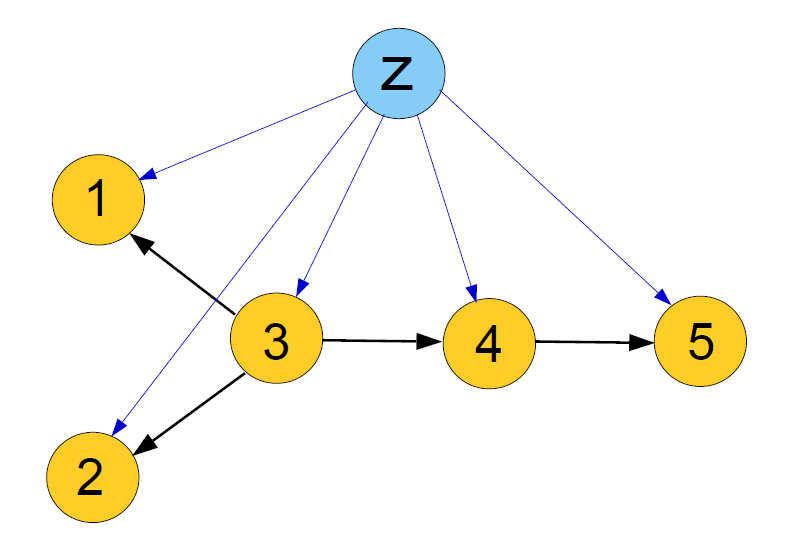
\includegraphics[width=0.4\textwidth]{MixtureOfTrees}
	\caption{A Mixture Of Trees. Courtesy:Heckerman, Et al.}
\end{figure}
\noindent The mixture of trees can be defined as:
\begin{equation}
Q(x)=\sum\limits_{k=1}^{m}\lambda_kT^k(x)
\end{equation}
with the constraint that 
\[\lambda_k\geq0,k=1,\ldots,m\quad\sum\limits_{k=1}^{m}\lambda_k=1\]
This basically means that more than one trees are proposed in the model, each one of the tree is denoted by $T^k(x)$, with the probability of $\lambda_k$. 
To learn this mixture of trees, suppose we are given a set of observations $\vec{X}=(X_1,X_2,\ldots,X_n)$, then the mixture of trees need to satisfy
\[Q=argmax\;\prod\limits_{i=1}^{N}Q(x_i)\]
Using the log-likelyhood, the equation becomes
\[Q=argmax\;\sum\limits_{i=1}^{N}\log{Q(x_i)}.\]
Now that we don't know the distribution of the mixture of trees, we will use the EM algorithm to calculate the likelihood. 
The conditional distribution of the mixture of trees can be calculated as:
\[\gamma_k(i)=\dfrac{\lambda_kT^k(x^i)}{\sum_{k'}\lambda_{k'}T^{k'}(x^i)}\]
Substituting this into the expectation of log-likelihood, we obtain
\begin{align*}
& E[(x^{1,\ldots,N},Q^{1,\ldots,m})]\\
& =\sum\limits_{i=1}^{N}\sum\limits_{k=1}^{m}\gamma_k(i)(\log\lambda_k+log{T^k(x^i)})
\end{align*}
With this formulation, we can take the maximum likelihood of the undetermined parameters by using the gradient methods. 

\noindent Using the mixture of trees, experiments are carried out, and it is observed that the mixture of trees has a better accuracy over methods like linear discrimination, Naive Bayes and Bayesian networks. In terms of computational cost, there is a slight increase on the efficiency using traditional algorithms. By taking advantage of the sparseness of the tree structures, a 5-7 times improvement on the efficiency is reported in the experiments. 
\section{Learning Probabilistic Decision Graphs}
In 2006, Jaeger\cite{jaeger2006learning} proposed a method to learn a probabilistic decision graph. A probabilistic decision graph is rooted on tree representations of distributions. Eachnode $X_i$ in the forest is expanded into a set $V_i$ of nodes. $v_i$ in the probabilistic decision graph is connected in the following manner: for each successor $X_j$ of $X_i$ in the tree, and each possible value of $X_i$ there is one outgoing edge connecting these two states. Basically each $V_i$ represent a node and each $v_j$ represent a state of the node, the line style (solid or dotted) connecting two $v_j$ represents value 1 or 0, respectively. Then the values in the node denotes the probability distribution over the possible states of $X_i$.
\begin{figure}[h!]
	\centering
	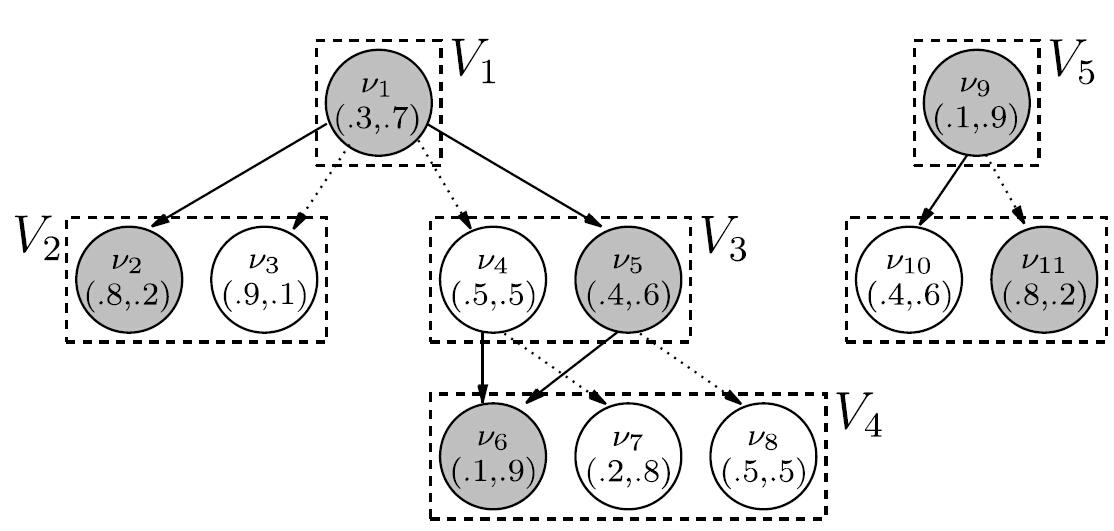
\includegraphics[width=0.4\textwidth]{ProbabilisticDistributionGraph}
	\caption{A probabilistic distribution graph. Courtesy:Jaeger, Et al.}
\end{figure}
\begin{figure}[h!]
	\centering
	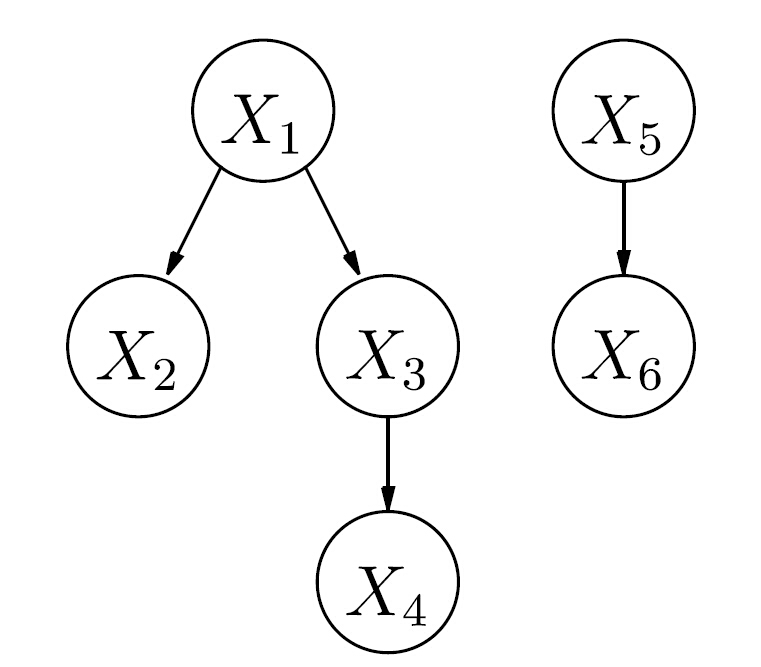
\includegraphics[width=0.2\textwidth]{Forests}
	\caption{A probabilistic distribution graph. Courtesy:Jaeger, Et al.}
\end{figure}
The probabilistic decision graph in Fig. 2 is based on the tree structure shown in Fig. 3.

Similar to the Bayesian networks, the efficiency of learning a probabilistic decision graph can be measured by the size of the PDG. It is reported that the results from applying the PDG method is very similar to the Bayesian networks. Some improvement of accuracy is observed with PDG over Bayesian networks, but the overall computational cost and complexity is very close. 

\section{Summary}
This report summarize the CS446 project of the author. In this project, the author conducted a survey of the machine learning history and its development. A short literature review for the comparison of some of the algorithms that are discussed in the course is also presented. Then author studied in-depth the multi-linear representations of distributions. Although some of the concepts is not well understood, the main idea and logic of the paper is studied and presented. The author also found two paper interesting and very well related to the concepts and algorithms discussed in class. These two papers focused on learning distributions with mixture of trees and learning probabilistic decision graph. The author went into details for the parts which has a connection with the algorithms discussed in the course.

The author felt learning quite a lot in both the course and the project. The project helps the author to have the feeling that what is discussed in the course is indeed the state-of-the-art of machine learning. Now that we are equipped with the essentials to enter this field, either as a personal interest or as a specialist. 

\bibliography{trycitation}
\end{document}
